\documentclass[tikz,border=8pt]{standalone}
\usepackage{tikz}
\usetikzlibrary{arrows.meta,positioning,fit}

\tikzset{
  layer/.style={
    draw,
    rounded corners=2pt,
    thick,
    align=center,
    minimum width=2.9cm,
    minimum height=1.15cm,
    font=\small,
    fill=blue!8
  },
  head/.style={
    layer,
    fill=green!10
  },
  io/.style={
    layer,
    fill=gray!12
  },
  flow/.style={
    -{Latex[length=2.6mm]},
    thick
  }
}

\begin{document}
\begin{tikzpicture}[node distance=0.95cm]
  \node[io] (input) {Input mel\\$1 \times M \times T$};
  \node[layer, right=of input] (conv1) {Conv2d\\$1 \rightarrow 8$\\$3 \times 3$, pad $1$};
  \node[layer, right=of conv1] (relu1) {ReLU};
  \node[layer, right=of relu1] (pool1) {MaxPool2d\\$2 \times 2$\\$8 \times \frac{M}{2} \times \frac{T}{2}$};
  \node[layer, right=of pool1] (conv2) {Conv2d\\$8 \rightarrow 16$\\$3 \times 3$, pad $1$};
  \node[layer, right=of conv2] (relu2) {ReLU};
  \node[layer, right=of relu2] (avg) {AdaptiveAvgPool2d\\output $4 \times 8$\\$16 \times 4 \times 8$};
  \node[head, right=of avg] (flat) {Flatten\\$512$};
  \node[head, right=of flat] (fc1) {Linear\\$512 \rightarrow 32$};
  \node[head, right=of fc1] (relu3) {ReLU};
  \node[head, right=of relu3] (drop) {Dropout\\$p=0.2$};
  \node[head, right=of drop] (fc2) {Linear\\$32 \rightarrow \mathrm{out\_dim}$};

  \draw[flow] (input) -- (conv1);
  \draw[flow] (conv1) -- (relu1);
  \draw[flow] (relu1) -- (pool1);
  \draw[flow] (pool1) -- (conv2);
  \draw[flow] (conv2) -- (relu2);
  \draw[flow] (relu2) -- (avg);
  \draw[flow] (avg) -- (flat);
  \draw[flow] (flat) -- (fc1);
  \draw[flow] (fc1) -- (relu3);
  \draw[flow] (relu3) -- (drop);
  \draw[flow] (drop) -- (fc2);

  \node[draw, dashed, rounded corners=3pt, inner sep=6pt, fit=(conv1)(avg), label=above:{\small Convolutional Trunk}] {};
  \node[draw, dashed, rounded corners=3pt, inner sep=6pt, fit=(flat)(fc2), label=above:{\small Classification Head}] {};
\end{tikzpicture}
\end{document}
